%!TEX root = ../main.tex

\section{Admission Protocol}
\label{sec:admission}

We now describe the registration procedure followed by an advertiser when attempting to register an advertisement (ad) at a specific registrar.

\subsection{Challenge}
Registrars have a limited amount of memory and can store only a finite number of ads. If the registration demand surpasses the supply each registrar has to decide which ads should be admitted. In an open setting, implementing simple replacement policies such as Least Recently Used (LRU) or Most recently used (MRU) exposes the system to an attacker that bombards registrars with dummy ads and evicts honest ones.

\sysname solves this problem by using a lightweight \textit{waiting-time-based admission mechanism} for access control. When an advertiser sends an ad placement request to a registrar, the registrar will calculate the amount of time the advertiser needs to wait before being admitted. This \emph{waiting time} is calculated based on the diversity of the request (\ie how different is the request from ads already in the registry) and the space left in the registry. We explain the waiting time calculations in \Cref{sec:waitingTime}. The advertiser must wait for a waiting time reported by the registrar before it is allowed to contact the registrar again and have its ad actually admitted.

\subsection{Data Structures}

\para{Advertisement}
When advertisers send a registration request, they send an \emph{advertisement}. The ad contains the IP address of the advertiser, the ID of the advertiser, the topic the ad is for and additional information needed to later contact the advertiser (\eg an application-specific port number). In the remaining part of the paper, we omit the additional information for brevity. 

\para{Ad cache}
Registrars store received ads locally in a data structure called an \emph{ad cache}. Each ad stored in the ad cache has an associated lifetime $a$, after which the ad is automatically removed. The total size of the ad cache is limited by $n$. \sysname does not impose topic/IP/ID-specific limits on the content of the \emph{ad cache} to accommodate for diverse network conditions and application popularity distributions.
A single advertiser may place at most one ad for a specific topic in the ad cache.
Registration requests for ads already in the cache are ignored.
An advertiser may, however, attempt to place ads for multiple topics at the same registrar.

\para{Ticket}
Tickets are immutable objects issued by registrars to advertisers when receiving a registration request. 
They are digitally signed by the issuing registrar.
Each ticket contains:
\begin{itemize}
    \item Ad - a copy of a registration request (as described above). 
    \item Initial timestamp - the local time at the registrar when the ad was received for the first time, $t_\textit{init}$
    \item Waiting time - the waiting time calculated by the advertiser for the ad, $t_\textit{waiting}$.
    % We describe the details of the waiting time calculations in \Cref{sec:waitingTime}. \er{already said}
\end{itemize}

% The tickets are digitally signed by the issuing registrar. \er{should we give more details here? What is the purpose? Do we assume the registrar knows the public key of the advertiser, always, so it can check this signature?}\mk{It was actually a mistake (now corrected). The ticket are signed by registrars (not advertisers). The registrars issues the ticket to the advertiser and signs it so that when the advertisers comes back, the registrar can verify the integrity of the ticket. It's kind of explained later, so not sure whether we should include more info here.}

\subsection{Registration Procedure}
An advertiser willing to register an ad at a registrar starts by sending an
initial request uniquely containing the ad itself. Based on the
content of the ad cache and the incoming registration, the registrar calculates an
ad-specific waiting time (as detailed in \Cref{sec:waitingTime}). 
The advertiser then issues a ticket including the calculated waiting time and the time of receiving the initial request and sends it back to the advertiser.

The advertiser waits for the indicated time and attempts to register again. The consecutive registration request must include the last ticket issued by the registrar. Tickets can be used uniquely during a registration window:
\begin{equation}\label{eq:registration_window}
    t_\textit{window} = [t_\textit{init} + t_\textit{waiting}, t_\textit{init} + t_\textit{waiting} + \delta t_\textit{window}]
\end{equation}
All registration requests outside the registration window are ignored by the advertiser. The registrar calculates the registration windows based on the content of the ticket. $\delta t_\textit{window}$ should be chosen to accommodate for the maximum delay between the advertiser and the registrar. The mechanism prevents an attacker from gathering many tickets, accumulating long waiting times (see below) and submitting the tickets all at once to overwhelm the registrar. 

The advertiser calculates a new waiting time, based on the current content of
the ad cache, every time it receives a registration request (with or without
a ticket). The waiting time in the ticket is used only to calculate the
registration windows and prevent advertisers from trying to register
continuously. The ticket also allows the calculation of an \emph{accumulated} waiting time:
\begin{equation}
    t_\textit{cumulative} = \textit{now} - t_\textit{init}
\end{equation}
An ad is admitted if, and only if, the accumulated waiting time is equal to or larger than the calculated waiting time $t_\textit{cumulative} \ge w$\footnote{Note that a registration request without a ticket may be admitted directly when the calculated waiting time equals $w=0$.}. For registration requests without a ticket $t_\textit{cumulative} = 0$. An advertiser that misses its registration window (as specified by the most recent ticket), loses all its cumulative waiting time and must attempt to re-register without a ticket. Once an ad is admitted, the registrar confirms the registration to the advertiser.

If the cumulative time is not sufficient, $t_\textit{accumulated} < t_\textit{waiting}$, the registrar issues a new ticket and the advertiser repeats the whole procedure. With consecutive registration attempts, advertisers increase their cumulative waiting time $t_\textit{cumulative}$ and eventually will be admitted. 


\begin{figure}
    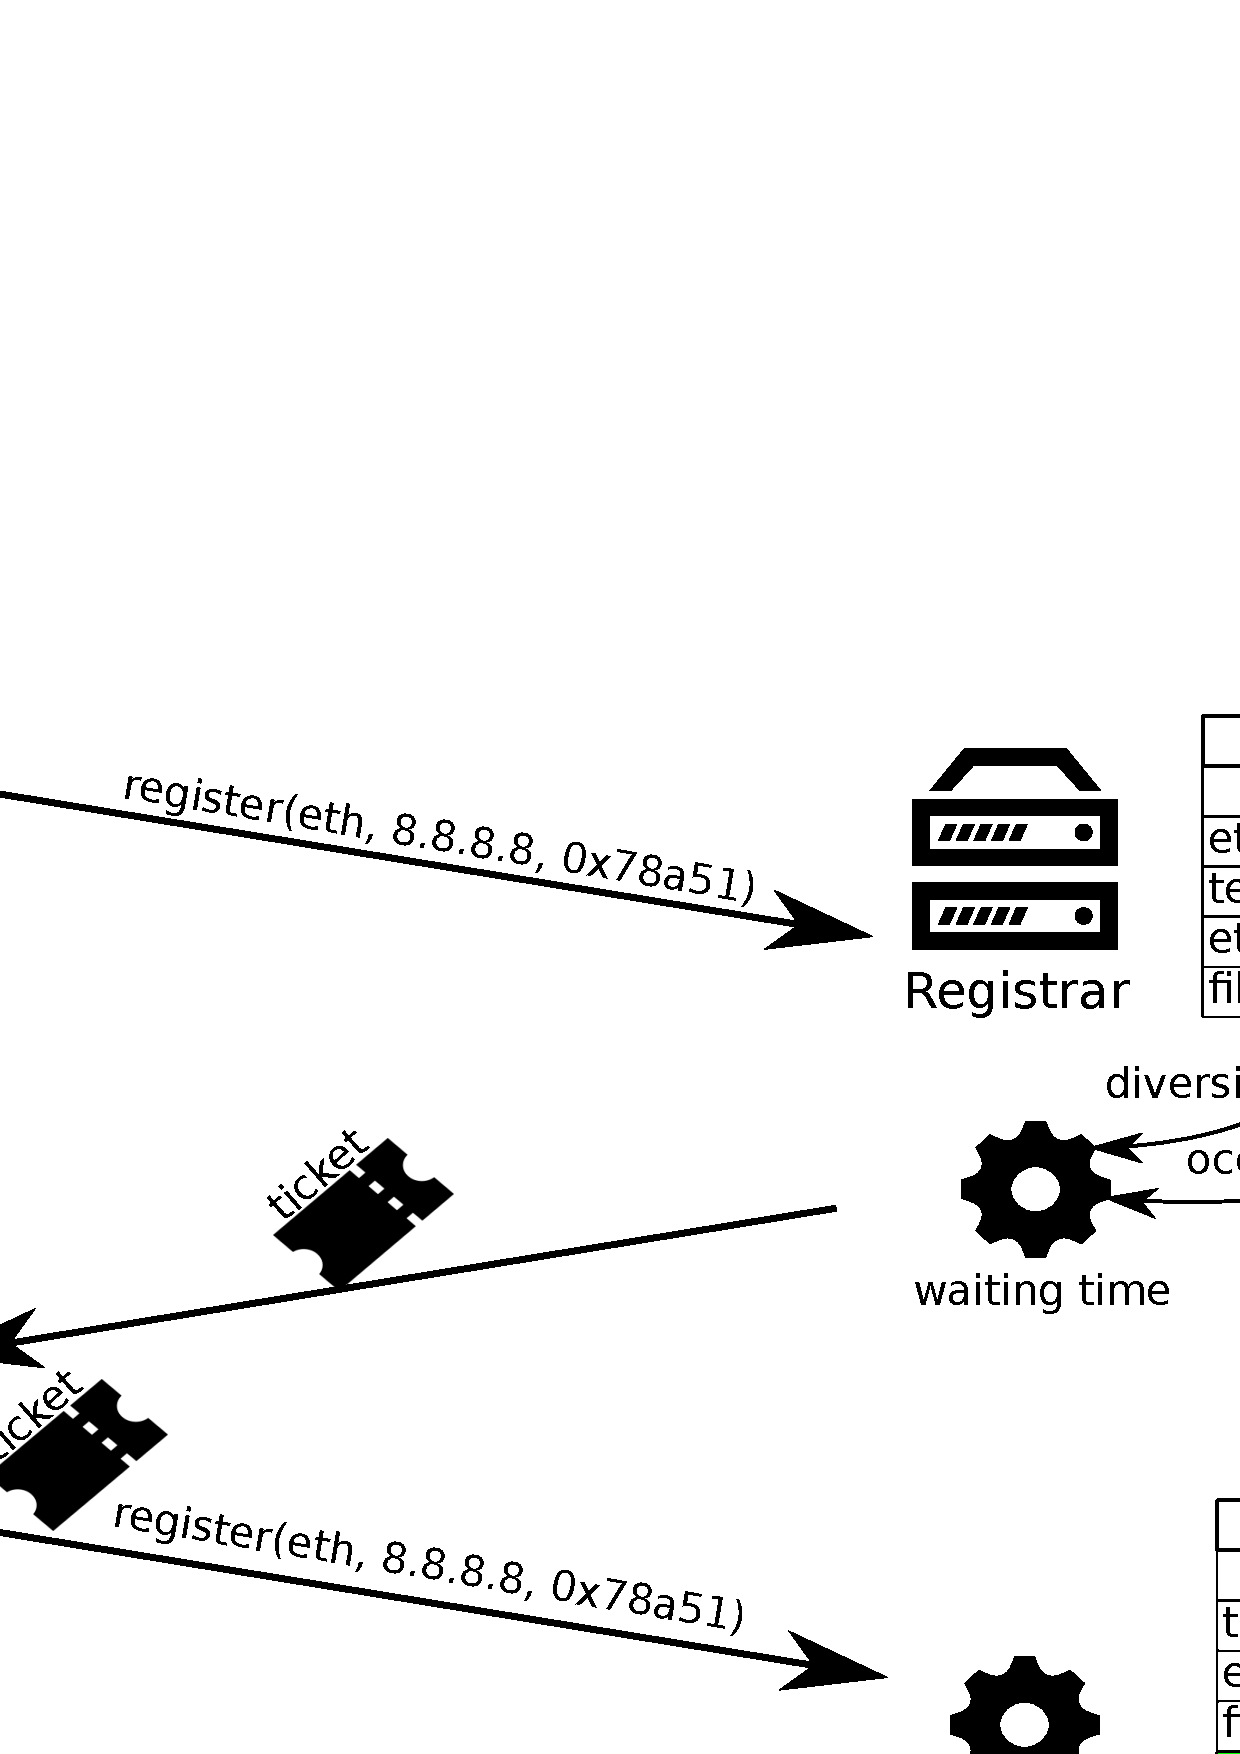
\includegraphics[width=0.45\textwidth]{img/registration}
    \vspace{-0.15in}
    \caption{Registration operation.}
    \label{fig:registration}
    \vspace{-0.15in}
\end{figure}

The inclusion of issue-time allows the registrars to prioritize advertisers that have been waiting for the longest time, as we explain later. The tickets are immutable (\ie, tampering with the ticket is detectable by the registrars that originally issued the ticket thanks to the digital signature). When a registrar issues a new ticket (in case registration is not immediately successful) to an advertiser, the registrar simply copies the issue-time from the last issued ticket and uses that as the issue-time of the new ticket. This means that the registrars are not required to maintain any state for each ongoing ticket request given that they can verify the authenticity of the ticket in the incoming registration requests.



An advertiser gives up and stops the registration process with a registrar when it has received $r$ unsuccessful registration attempts (i.e., after being issued $r$ tickets without being admitted). In this case, the advertiser removes the registrar from its advertise table and selects a new node located in the same bucket and attempts a new registration procedure. The mechanism prevents malicious registrars from stalling honest advertisers.
%\michal{Is the below true? Shouldn't we try to register at the same node?}
%\sergi{We dont use the same, we pick another randomly. we could use the same but i think for diversity could be better  this way}
Similarly, after the expiration of a previously placed ad, the registrar is removed from the advertise table and the process is restarted with a new node picked from the local route table.%\footnote{We assume a common expiration time for all the registrar. However, each registrar may choose to implement its own expiration time and communicate it to advertisers in the confirmation message}.
